\documentclass[10pt]{article}

% Your language, here German
\usepackage[ngerman]{babel} 
% Will work with Umlauts
\usepackage[utf8]{inputenc}
% Euro characters etc.
\usepackage{textcomp}
% Works perfectly with latin1
\usepackage{listings}

\usepackage[T1]{fontenc}
\usepackage{ae,aecompl}

% Set Page Size
\usepackage[a4paper]{geometry}

% Support for PDF inclusion
\usepackage[final]{pdfpages}

% Support for PDF scaling
\usepackage{graphicx}


\lstset{% Default options for all algorithm listings read
  %labelstep=5,
  %frame=trbl,
  %indent=15pt,
  %indent=12pt,
  breaklines=true,
  numbers=left,
  numberstyle=\tiny,
  showlines=false,
  showstringspaces=false,
  stepnumber=2,
  stringstyle=\itshape,
  commentstyle=\color{red},
  keywordstyle=\bfseries\color{blue},
  %basicstyle=\ttfamily\footnotesize
}
\geometry{a4paper, portrait, left=1.5cm, right=1cm, top=2cm, bottom=2cm}
\newcommand{\mylisting}[2][]{%
    \lstinputlisting[caption={\texttt{\detokenize{#2}}},#1]{#2}%
}


\begin{document}
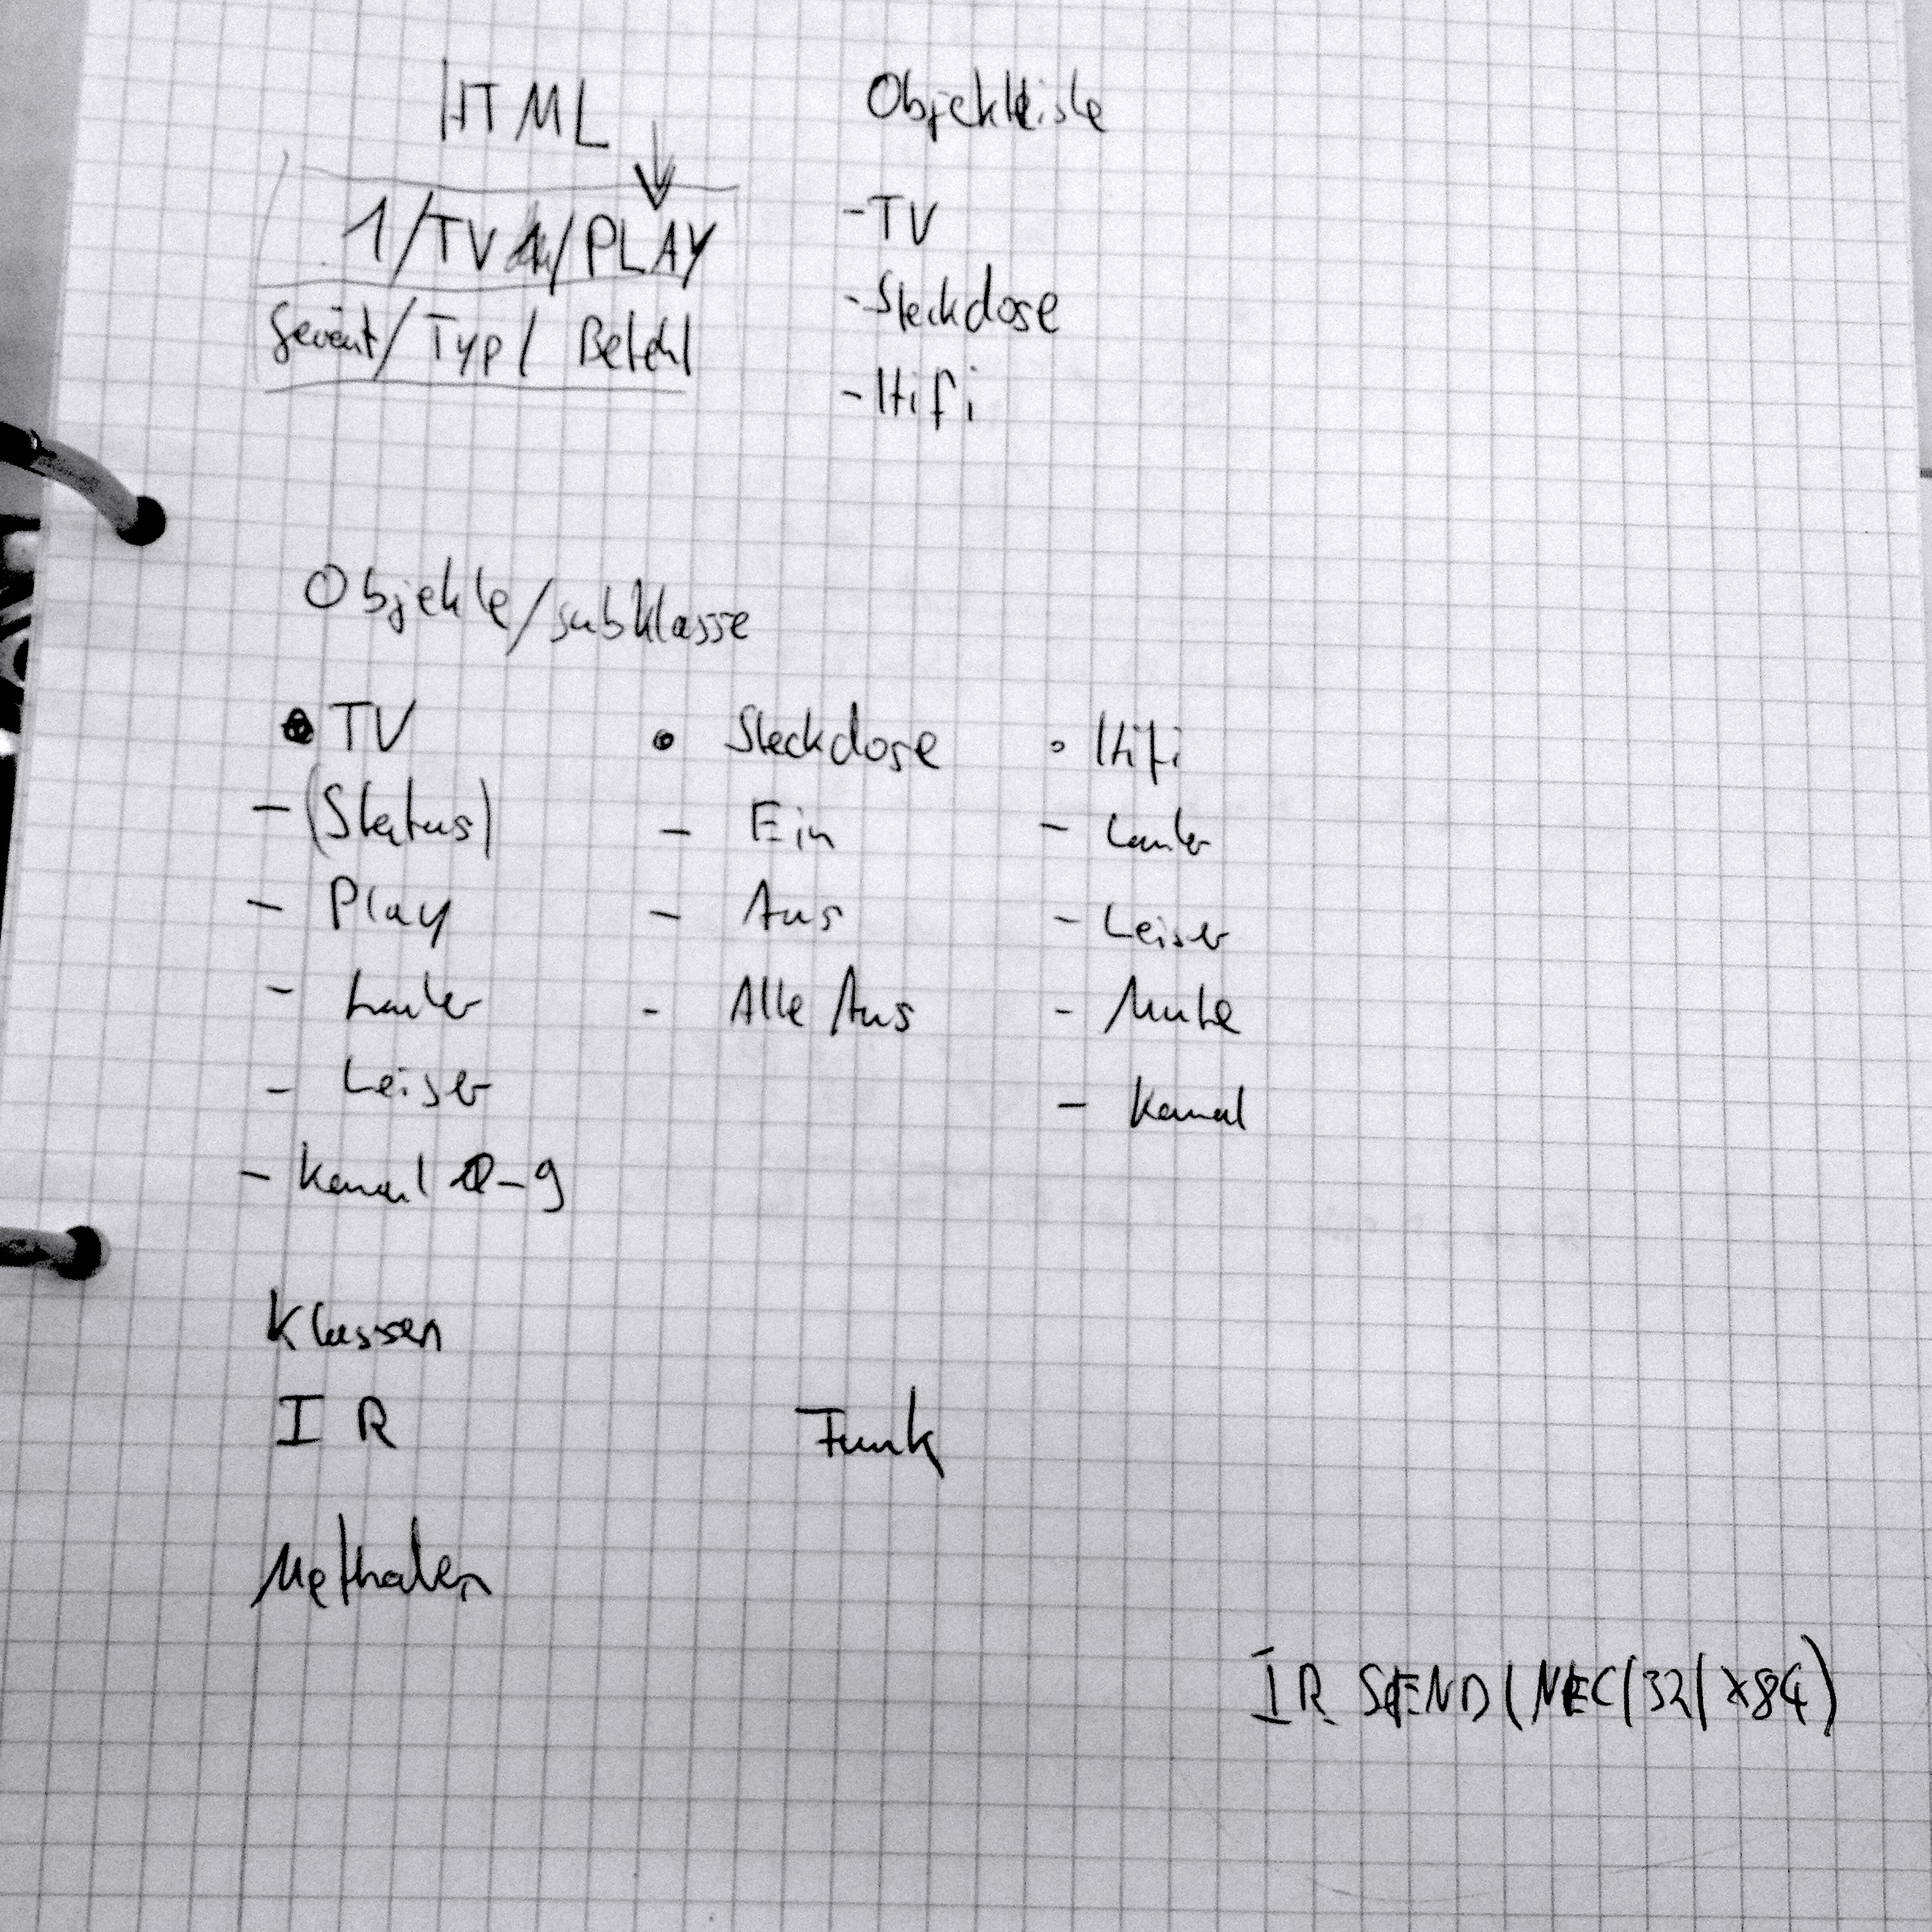
\includegraphics[width=\textwidth]{images/Stuktur-Sketch.jpg}


% Globals: include all pages, don't auto scale
\includepdfset{pages=-,noautoscale}

% Include the PDF files, scaling as required
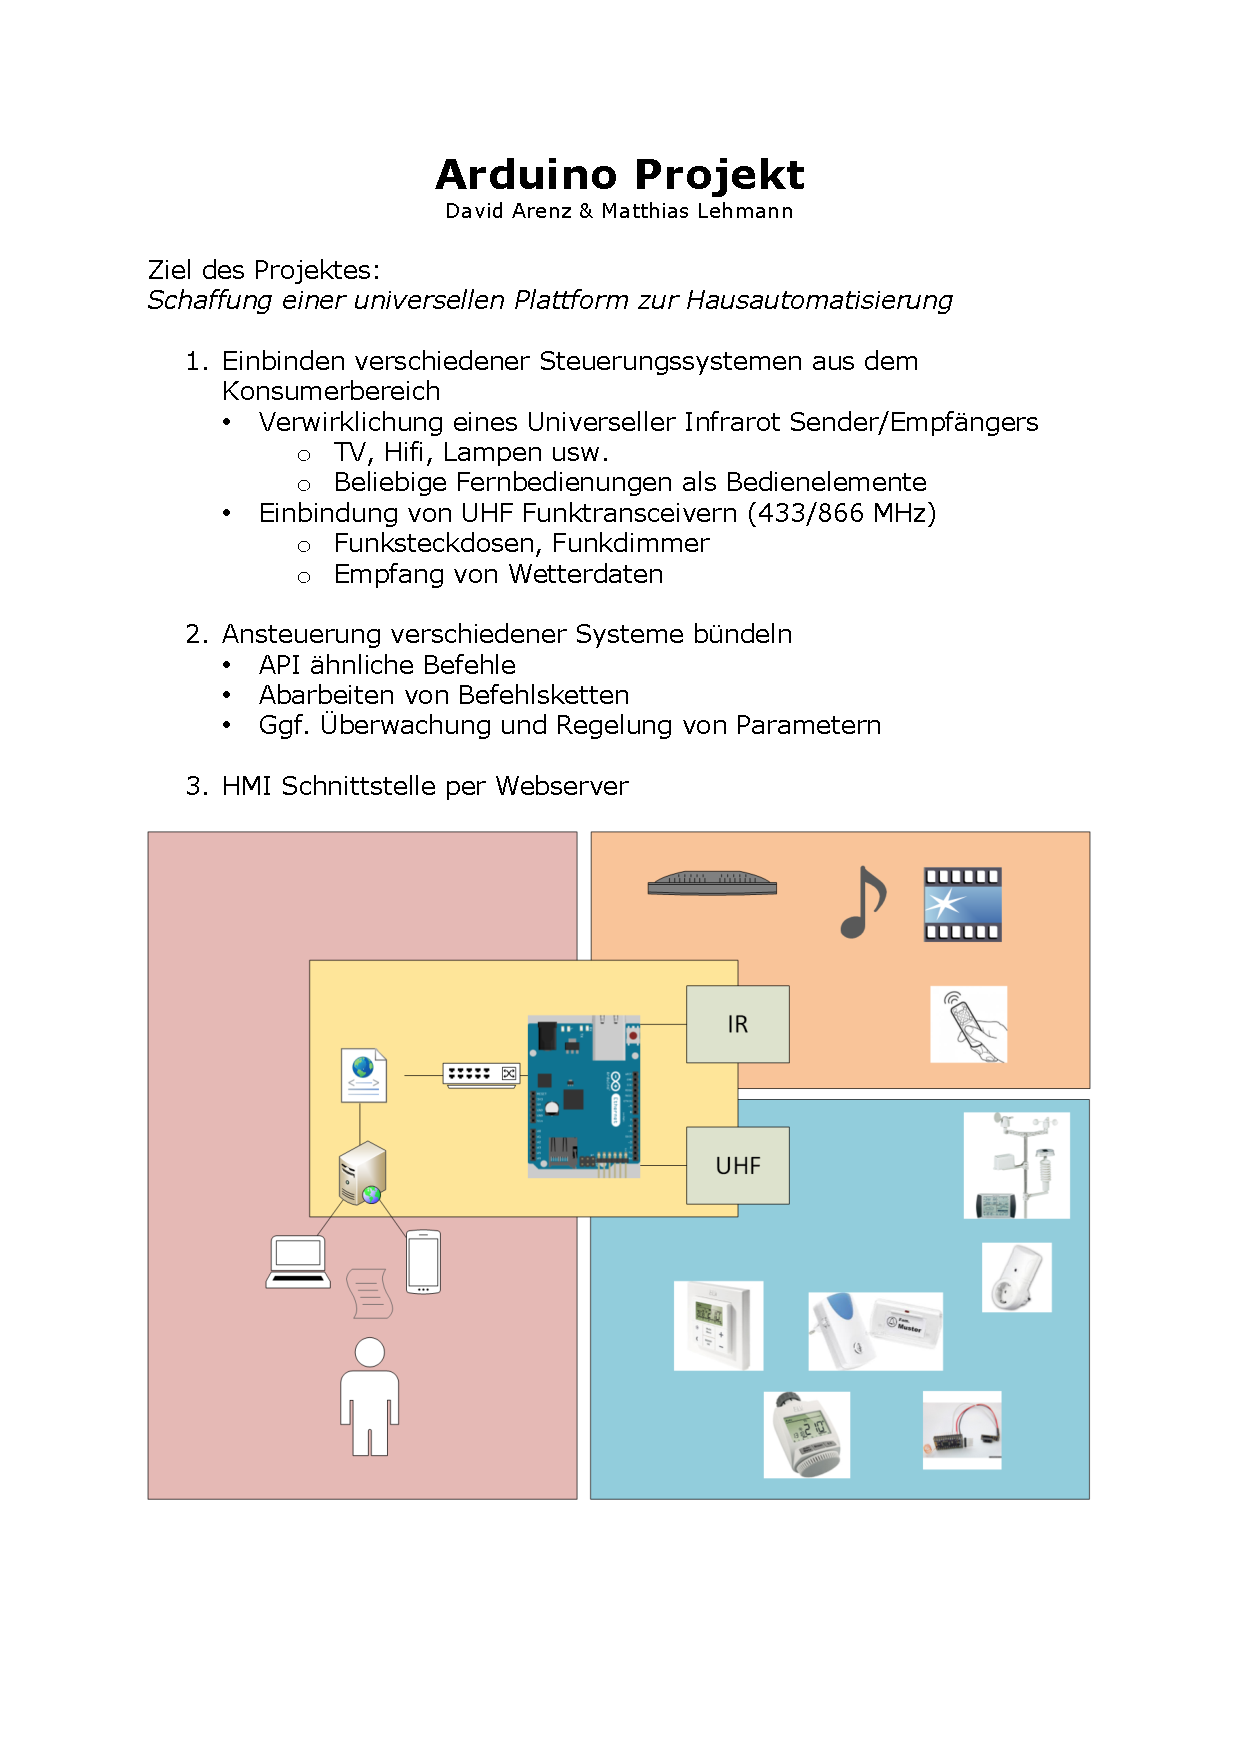
\includepdf{Arduino-Projekt-Overview.pdf}

\section{Troubleshoting}

\begin{itemize}
\item Fehler: Initialisierung der SD-Karte fehlgeschlagen!
\subitem Ursache: Die SD Karte ist nach dem Laden eines neuen Sketches noch initialisiert. Ein normaler Reset reicht scheinbar nicht aus.

\subitem Loesung: SD Karte komplett entfernen, SD Karte einstecken, 3s lang den REST Button druecken

\item Symptom: Keine Ausgabe auf der Konsole.
\subitem Fehler:  Arduino bekommt keine IP (vermutlich)
\subitem Loesung:
\begin{itemize}
	\item Konsole schliessen
	\item Arduino von USB und NW trennen
	\item NW anschliessen
	\item USB anschliessen
	\item Arduino reseten
	\item Konsole oeffnen
\end{itemize}
\end{itemize}

Important Note!

If an uninitialized SD card is left in the SD card socket of the shield, it can cause problems with code in the sketch that is accessing the Ethernet chip. This may cause symptoms such as the sketch running once or twice, then hanging up.

This is because both the Ethernet chip and the SD card are accessed by the Arduino using the same SPI bus.

If the SD card is not being used with an Ethernet application, either remove it from the socket or add the following code to disable the SD card:

\section{Code}
\subsection{WEB\_SD\_IR.ino}
	\mylisting[language=C]{../code/WEB_SD_IR/WEB_SD_IR.ino}
\newpage
\section{Beispiele}
\subsection{InfraredDumper.ino}
	\mylisting[language=C]{../example/InfraredDumper/InfraredDumper.ino}
\newpage
\subsection{InfraredProxy.ino}
	\mylisting[language=C]{../example/InfraredProxy/InfraredProxy.ino}
%\subsection{SDWebServer.ino}
%	\mylisting[language=C]{../example/SDWebServer/SDWebServer.ino}
	

\end{document}